\documentclass[a4paper,11pt]{article}
\usepackage[UTF8]{ctex}
\usepackage{pdfpages}
\usepackage{zh_CN-Adobefonts_external}
\usepackage{geometry}
\usepackage{fancyhdr}
\usepackage{minted}
\usepackage[colorlinks,
linkcolor=black,CJKbookmarks,
]{hyperref}
\usepackage[T1]{fontenc}
\usepackage[utf8]{inputenc}
\setlength{\headheight}{15pt}
\pagestyle{fancy}
\fancyhf{}
\fancyhead[C]{ACM Templates by XTS}
\lfoot{}
\cfoot{\thepage}
\rfoot{}

\author{XTS}
\title{ACM Templates}
\hyphenpenalty=500000
\tolerance=10
\geometry{a4paper,left=2cm,right=2cm,top=3cm,bottom=3cm}
\begin{document}
    \maketitle
    \newpage
    \tableofcontents




    \newpage
    \section{图论} % 一级标题

    \subsection{dijstra}
    \inputminted[breaklines]{c++}{Graph/dijstra.cpp}

    \subsection{倍增LCA}%三级标题
    \inputminted[breaklines]{c++}{Graph/lca.cpp}

    \subsection{树上路径交}
    \inputminted[breaklines]{c++}{Graph/树上路径交.cpp}

    \subsection{树链剖分}
    \inputminted[breaklines]{c++}{Graph/树链剖分.cpp}

    \subsection{点分治}
    \inputminted[breaklines]{c++}{Graph/点分治.cpp}

    \subsection{强连通分量}
    \inputminted[breaklines]{c++}{Graph/scc.cpp}

    \subsection{双连通分量}
    \inputminted[breaklines]{c++}{Graph/bcc.cpp}

    \subsection{仙人掌求环}
    \inputminted[breaklines]{c++}{Graph/仙人掌求环.cpp}

    \subsection{dfs判负环}
    \inputminted[breaklines]{c++}{Graph/dfs判负环.cpp}

    \subsection{斯坦纳树}
    \inputminted[breaklines]{c++}{Graph/斯坦纳树.cpp}
    
    \subsection{二分图最大匹配}
    \inputminted[breaklines]{c++}{Graph/二分图最大匹配.cpp}

    \subsection{二分图最大权匹配}
    \inputminted[breaklines]{c++}{Graph/KM.cpp}

    \subsection{最大流}
    \inputminted[breaklines]{c++}{Graph/Dinic.cpp}

    \subsection{最小割树}
    \inputminted[breaklines]{c++}{Graph/最小割树.cpp}
    
    \subsection{费用流}
    \inputminted[breaklines]{c++}{Graph/费用流.cpp}
    
     \subsection{zkw费用流}
    \inputminted[breaklines]{c++}{Graph/zkw费用流.cpp}
    
    \subsection{网络流的一些结论}
    
    \paragraph{S集}割出的两个点集中和S相连的那个,即为Dinic算法最后增广失败后所有被标号(d不为0)的点
     \paragraph{T集}割出的两个点集中和T相连的那个,即为Dinic算法最后增广失败后所有未被标号(d不为0)的点
     \paragraph{最小割的方案输出问题}
     \ 
     
     \textbf{可在最小割上的边}
     
     做完网络流后,求残量网络 SCC。 
     设点 x 所在 SCC 编号为 SCC[x]。 
     对于满流边 ( u,v ),若 SCC[u]≠SCC[v]
     ,则边 ( u,v ) 可以在最小割上。
     
     原因: 将 SCC 缩点,那么新图的任意最小割都是原图的最小割,其中肯定有把 SCC[u] 和 SCC[v] 割开的最小割。
     
     \textbf{最小割的必须边}
     
     求残量网络 SCC。 
     对于满流边 ( u,v ) ,若 SCC[u]=SCC[S] 而且 SCC[v]==SCC[T] ,那么边 ( u,v ) 必须。
     
     原因: 如果一条边是必须的,那么增加这条边的容量一定会改变最大流。 
     残量网络的 SCC 缩点后构成一个 DAG ,其中 T 必然能到达 S ,总体方向是从 T 往 S 的方向连边。 
     当且仅当 ( u,v ) 刚好在 SCC[S] 和 SCC[T] 之间时,增加 ( u,v ) 的流量才能增大最大流。
     
     \textbf{最小割任意方案}
     
     每次选取一条满流边 ( u,v ) ,用一次 DFS 判断是否能在残量网络上,从 v 到达 u ,且不经过 ( u,v ) 的反向边。 
     如果不可以,那么 ( u,v ) 不在最小割集上,跳过。 
     如果可以,输出 ( u,v ) 。 
     当然,直接求SCC也是可以的,但是下一步需要O(n)的时间,所以这一步优化意义不大
     
     选了 ( u,v ) 之后,可能某些满流边再选就不是最小割了。 
     所以要消除 ( u,v ) 的影响。
     
     考虑强行退流 ( u,v ) 。 
     完全退流 ( u,v ) 相当于跑了一次 EK,不优。 
     但是我们不需要完全退流,只需要退流 1 即可。
     
     退流 1 的方法是:从 T 开始 DFS 到 v ,找一条路流 1 。 
     然后从 u 开始 DFS 到 S , 找一条路径流 1 。 
     然后把 ( u,v ) 及其反向边删掉。(即容量设为 0)
     
     这样就改变了原图的连通性,让不能再选的边不再满流或者不在最小割集上。
     
     \textbf{最小字典序最小割方案}
     
     同上,从编号小的边开始枚举。
     
     \textbf{最少割边的最小割方案}
     
     做完一次最小割后,令所有满流边容量为 1,非满流边容量为 ∞ 。
     再做一次最小割,此时的任意最小割方案割边都最少。
     
     \textbf{最少割边字典序最小最小割方案}
     
     总和以上,先做一次最小割,按照最少割边的方式处理后再做一次,再跑最小字典序的最小割方案。
    
	\paragraph{最大闭合子图}
	带点权的有向图的最大子图,使得子图中所有点的出边都指向子图内的点。
	
	正权点连S流量为点权,负权点连T流量为点权的绝对值,原图的边流量为INF,跑最大流,正权点和减去最大流即为答案。S集中的点形成了最大闭合子图。
    
    \paragraph{DAG最少路径覆盖}
    找出最少的路径,使得这些路径经过了所有的点。
    
    最少不相交路径覆盖:把原图的每个点V拆成Vx和Vy两个点,如果有一条有向边A->B,那么就加边Ax−>By。这样就得到了一个二分图。那么最小路径覆盖=原图的结点数-新图的最大匹配数。其中每个从Ax->By的匹配代表让A成为原本以B为起点的路径的新起点。
    
   	最少可相交路径覆盖:对原图做floyd传递闭包,若A能到达B则建边AB,对新图做最少不相交路径覆盖。
   	
   \paragraph{二分图 最小点覆盖=最大匹配=总点数 - 最大独立集 (带点权同理 但只能用最大流做)}
   	






    \newpage
    \section{字符串}

    \subsection{回文树}
    \inputminted[breaklines]{c++}{String/pam.cpp}

    \subsection{广义后缀自动机}
    \inputminted[breaklines]{c++}{String/sam.cpp}

    \subsection{kmp}
    \inputminted[breaklines]{c++}{String/kmp.cpp}


    \newpage
    \section{数据结构}











    \newpage
    \section{数学} % 一级标题

    \subsection{带预处理BGSG}
    \inputminted[breaklines]{c++}{Math/BGSG.cpp}

    \subsection{十进制矩阵快速幂}
    \inputminted[breaklines]{c++}{Math/快速幂.cpp}

    \subsection{exlucas}
    \inputminted[breaklines]{c++}{Math/exlucas.cpp}

    \subsection{BM}
    \inputminted[breaklines]{c++}{Math/BM.cpp}

    \subsection{杜教筛}
    \inputminted[breaklines]{c++}{Math/杜教筛.cpp}

    \subsection{线性基}
    \inputminted[breaklines]{c++}{Math/线性基.cpp}

    \subsection{原根}
    \includepdf[pages={1}]{Math/原根.pdf}

    \subsection{欧拉降幂}
    \inputminted[breaklines]{c++}{Math/欧拉降幂.cpp}

    \subsection{拉格朗日插值}
    \includepdf[pages={1,2}]{Math/拉格朗日插值.pdf}

    \subsection{伯努利数}
    \includepdf[pages={1,2}]{Math/伯努利数.pdf}

    \subsection{FFTNTTFWT}
    \includepdf[pages={1,2,3,4,5,6}]{Math/FFTNTTFWT.pdf}


    \newpage
    \section{杂项}

    \subsection{约瑟夫问题}
    \includepdf[pages={1,2,3}]{Others/约瑟夫问题.pdf}

    \subsection{RSA}
    \includepdf[pages={1}]{Others/RSA.pdf}

    \subsection{快速读}
    \inputminted[breaklines]{c++}{Others/quick_IO.cpp}

    \subsection{并没有任何用处的卡常小知识}
    \inputminted[breaklines]{c++}{Others/并没有任何用处的卡常小知识.cpp}

    \subsection{杂杂杂项}
    \includepdf[pages={1,2,3,4,5,6,7}]{Others/推导用.pdf}

    \subsection{pbds}
    \includepdf[pages={1-14}]{Others/pbds.pdf}
    
     \subsection{线段覆盖专题}
    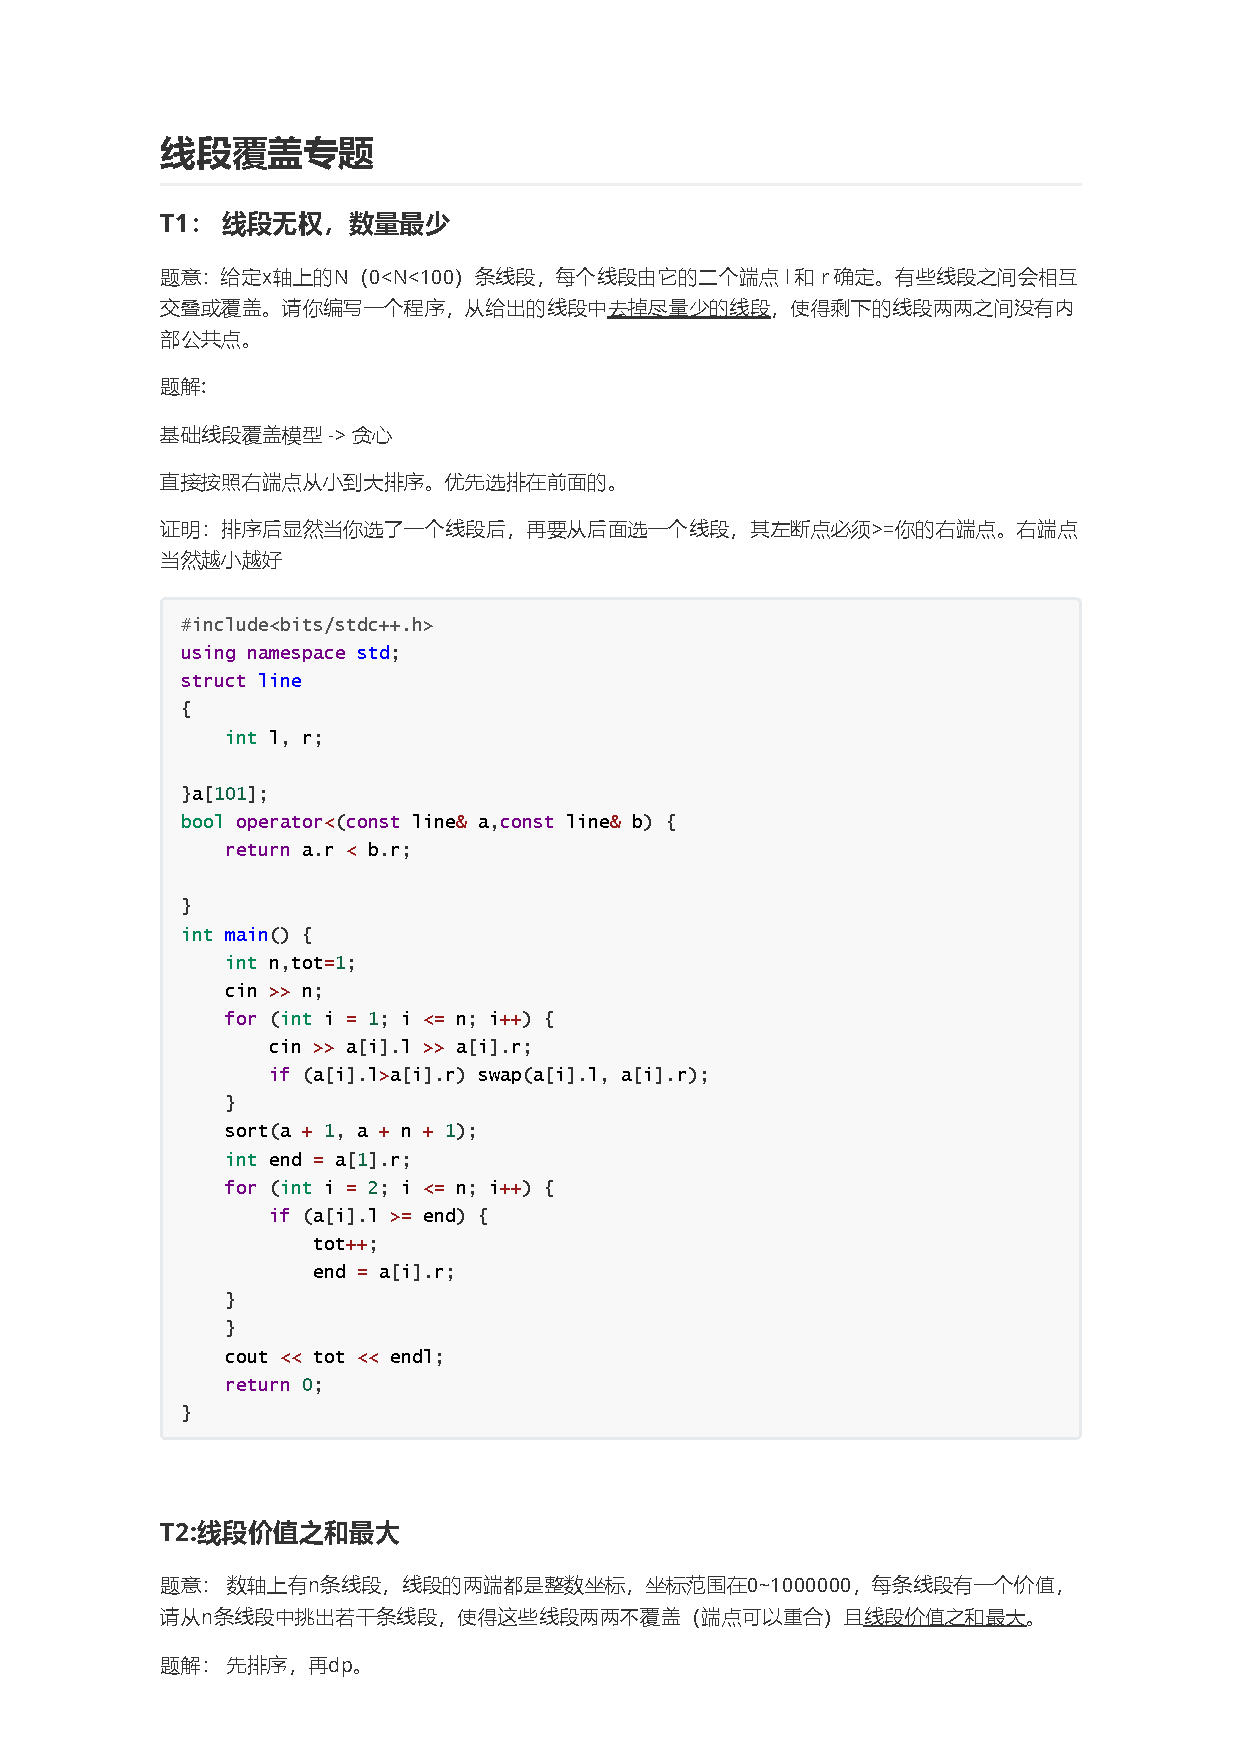
\includepdf[pages={1-6}]{Others/线段覆盖专题.pdf}




    \newpage
    \section{计算几何}


    %\newpage
    %\section{Others}

\end{document}


